\PassOptionsToPackage{unicode=true}{hyperref} % options for packages loaded elsewhere
\PassOptionsToPackage{hyphens}{url}
%
\documentclass[]{article}
\usepackage{lmodern}
\usepackage{amssymb,amsmath}
\usepackage{ifxetex,ifluatex}
\usepackage{fixltx2e} % provides \textsubscript
\ifnum 0\ifxetex 1\fi\ifluatex 1\fi=0 % if pdftex
  \usepackage[T1]{fontenc}
  \usepackage[utf8]{inputenc}
  \usepackage{textcomp} % provides euro and other symbols
\else % if luatex or xelatex
  \usepackage{unicode-math}
  \defaultfontfeatures{Ligatures=TeX,Scale=MatchLowercase}
\fi
% use upquote if available, for straight quotes in verbatim environments
\IfFileExists{upquote.sty}{\usepackage{upquote}}{}
% use microtype if available
\IfFileExists{microtype.sty}{%
\usepackage[]{microtype}
\UseMicrotypeSet[protrusion]{basicmath} % disable protrusion for tt fonts
}{}
\IfFileExists{parskip.sty}{%
\usepackage{parskip}
}{% else
\setlength{\parindent}{0pt}
\setlength{\parskip}{6pt plus 2pt minus 1pt}
}
\usepackage{hyperref}
\hypersetup{
            pdftitle={A Standardized Effect Size for Evaluating the Comparing the Strength of Phylogenetic Signal},
            pdfborder={0 0 0},
            breaklinks=true}
\urlstyle{same}  % don't use monospace font for urls
\usepackage[margin=1in]{geometry}
\usepackage{longtable,booktabs}
% Fix footnotes in tables (requires footnote package)
\IfFileExists{footnote.sty}{\usepackage{footnote}\makesavenoteenv{longtable}}{}
\usepackage{graphicx,grffile}
\makeatletter
\def\maxwidth{\ifdim\Gin@nat@width>\linewidth\linewidth\else\Gin@nat@width\fi}
\def\maxheight{\ifdim\Gin@nat@height>\textheight\textheight\else\Gin@nat@height\fi}
\makeatother
% Scale images if necessary, so that they will not overflow the page
% margins by default, and it is still possible to overwrite the defaults
% using explicit options in \includegraphics[width, height, ...]{}
\setkeys{Gin}{width=\maxwidth,height=\maxheight,keepaspectratio}
\setlength{\emergencystretch}{3em}  % prevent overfull lines
\providecommand{\tightlist}{%
  \setlength{\itemsep}{0pt}\setlength{\parskip}{0pt}}
\setcounter{secnumdepth}{0}
% Redefines (sub)paragraphs to behave more like sections
\ifx\paragraph\undefined\else
\let\oldparagraph\paragraph
\renewcommand{\paragraph}[1]{\oldparagraph{#1}\mbox{}}
\fi
\ifx\subparagraph\undefined\else
\let\oldsubparagraph\subparagraph
\renewcommand{\subparagraph}[1]{\oldsubparagraph{#1}\mbox{}}
\fi

% set default figure placement to htbp
\makeatletter
\def\fps@figure{htbp}
\makeatother

\usepackage{setspace}\doublespacing
\usepackage{lineno}\linenumbers

\title{A Standardized Effect Size for Evaluating the Comparing the Strength of
Phylogenetic Signal}
\author{}
\date{\vspace{-2.5em}}

\begin{document}
\maketitle

\begin{center}
\textbf{Dean C. Adams$^{1 *}$, Erica K. Baken$^{1,2}$,  and Michael L. Collyer$^{2}$}
\end{center}

\begin{center}12 July, 2020\end{center}

\(^{1}\)Department of Ecology, Evolution, and Organismal Biology, Iowa
State University, Ames, Iowa, USA.

\(^{2}\)Department of Science, Chatham University, Pittsburgh,
Pennsylvania, USA.

\(^{*}\)Correspondence: Dean C. Adams
\href{mailto:dcadams@iastate.edu}{\nolinkurl{dcadams@iastate.edu}}
\hfill\break

\textbf{Keywords}: phylogenetic signal, lambda, kappa \hfill\break

\textbf{Short Title}: Effect size for phylogenetic signal \hfill\break

\begin{longtable}[]{@{}rr@{}}
\toprule
words & characters\tabularnewline
\midrule
\endhead
1751 & 10974\tabularnewline
\bottomrule
\end{longtable}

\newpage

\hypertarget{abstract}{%
\section{Abstract}\label{abstract}}

Macroevolutionary studies frequently characterize the phylogenetic
signal in phenotypes, and wish to compare the strength of that signal
across traits. However, analytical tools for such comparisons have
largely remained underdeveloped. In this study, we evaluated the
efficacy of one commonly used parameter (Pagel's \(\lambda\)) to
estimate the strength of phylogenetic signal in phenotypic traits, and
evaluate the degree to which \(\lambda\) correctly identifies known
levels of phylogenetic signal. We find that the precision of \(\lambda\)
in estimating actual levels of phylogenetic signal is often inaccurate,
and that biological interpretations of the strength of phylogenetic
signal based on \(\lambda\) are therefore compromised. We then propose a
standardized effect size based on \(\kappa\) (\(Z_\kappa\)), which
measures the strength of phylogenetic signal, and places it on a common
scale for statistical comparison. Tests based on \(Z_\kappa\) provide a
mechanism for formally comparing the strength of phylogenetic signal
across datasets, in much the same manner as effect sizes may be used to
summarize patterns in quantitative meta-analysis. Our approach extends
the phylogenetic comparative toolkit to address hypotheses that compare
the strength of phylogenetic signal between various phenotypic traits,
even when those traits are found in different evolutionary lineages or
have different units or scales.

\newpage

\hypertarget{introduction}{%
\section{Introduction}\label{introduction}}

Investigating macroevolutionary patterns of trait variation requires a
phylogenetic perspective, because the shared ancestry among species
violates an assumption of independence among trait values that is common
for statistical tests (1, 2). Accounting for this evolutionary
non-independence is the purview of \emph{phylogenetic comparative
methods} (PCMs): a suite of analytical tools that condition trends in
the data on the phylogenetic relatedness of observations (3--6). The
past several decades have witnessed an impressive expansion in the
development of PCMs to address an ever-growing set of macroevolutionary
hypotheses (7--13). These methods are predicated on the notion that
phylogenetic signal -- the tendancy for closely related species to
display similar trait values -- is present in cross-species datasets (1,
14, 15). Indeed, under numerous evolutionary models, phylogenetic signal
is to be expected, as stochastic character change along the hierarchical
structure of the tree of life generates trait covaration among related
taxa (1, 15, 16). \hfill\break

Several analytical tools have been developed to quantify phylogenetic
signal in phenotypic datasets, including measures of serial independence
(17), autocorrelation estimates (18), statistical ratios of trait
variation relative to what is expected given the phylogeny (12, 15), and
scaling parameters used in maximum likelihood fitting of the data to the
phylogeny (14), among others (19). The statistical properties of these
methods -- namely type I error rates and statistical power -- have also
been investigated to determine under what conditions phylogenetic signal
can be detected (12, 16, 20--24). One of the most widely used methods
for characterizing phylogenetic signal in macroevolutionary studies is
Pagel's \(\lambda\) (14). The parameter (\(\lambda\)) transforms the
lengths of the internal branches of the phylogeny to improve the fit of
data to the phylogeny via maximum likelihood (14, 25). Blomberg's
\(\kappa\) (15) is also widely used. This statistic measures the ratio
of trait variation to the amount expected under a Brownian motion (BM)
model of evolution. Pagel's \(\lambda\) and Blomberg's \(\kappa\) have
some similar intuitive appeal, namely because for both a value of \(0\)
corresponds to no phyloegentic signal in the data and a value of \(1\)
corresponds to the amount of phylogenetic signal one would expect with a
BM model of evolution. However, as putative measures (statistics) of the
amount of phylogenetic signal, they are calculated quite differently.
\hfill\break

In PGLS analysis, Pagel's \(\lambda\) is a parameter that ranges from
\(0\) to \(1\) and is optimized via log-likelihood profiling. After
obtaining an optimized \(\lambda\) value, \(\hat{\lambda}\), likelihood
ratio tests can be performed to compare observed model fits using
\(\hat{\lambda}\) to those obtained when \(\lambda=0\) or \(\lambda=1\)
to infer whether phylogenetic signal differs from no signal or a BM
model of evolutionary divergence, respectively (25--27). Confidence
limits on \(\hat{\lambda}\) can also be estimated based on percentiles
of a \(\chi^2\) distribution and where these values are mapped onto a
log-likelihood profile (25). With respect to confidence limits, one can
ascertain whether \(\lambda=0\) or \(\lambda=1\) is contained within an
interval of \(\hat{\lambda}\), as an analog to likelihood ratio tests
(28). It is, therefore, tempting to regard \(\hat{\lambda}\) as a
descriptive statistic that measures the relative strength of
phylogenetic signal, for inferring the extent to which shared
evolutionary history has influenced trait covariation among taxa. By
contrast, Blomberg's \(\kappa\) is a descriptive statistic that measures
the ratio of obsrved trait variation to the amount expected under a BM
model of evolution. Like Pagel's \(\lambda\), the range of \(0\) to
\(1\) defines a greater dependence of observed trait variation on the
phylogeny but values greater than 1 are possible when phylogenetic
signal is especially strong. Additionally, Blomberg's \(\kappa\) can be
a test statistic, by employing a permutation test to generate its
sampling distribution (12). Therefore, both statistics have a
descriptive meaning, plus an associated test for the null hypothesis of
no phlogenetic signal. An important question that has yet to considered
is whether these statistics are or can be converted to effect sizes for
comparative analyses? \hfill\break 

The appeal of either Pagel's \(\lambda\) or Blomberg's \(\kappa\) as
descriptive statistics is that they provide a basis for interpreting
``weak'' versus ``strong'' phylogenetic signal; i.e., small versus large
values of \(\hat{\lambda}\) or \(\kappa\), respectively, in a
comparative sense (29--31). As statistics, they should have reliable
distributional properties, which could be revealed with simulation
experiments. As a proportional random variable bounded by 0 and 1, we
might expect that \(\hat{\lambda}\) follows a Bernoulli distribution
(\textbf{add ref}); i.e., branch lengths in a tree are scaled
proportionally to the probability that data arise from a BM process. As
such, we would also expect in a simulation experiment that given a known
\(\lambda\) value used to generate random data on a tree that the mean
of an empirical sampling distribution of \(\hat{\lambda}\) would
approximately equal \(\lambda\); the dispersion of \(\hat{\lambda}\)
would be largest at intermediate values of \(\lambda\), and predictable
over the range of \(\lambda\) with respect to treesize; the distribution
of \(\hat{\lambda}\) would be symmetric at intermediate values of
\(\lambda\) and more skewed toward values of 0 or 1; and that the
distribution of \(\hat{\lambda}\) will be more platykurtic at
intermediate values of \(\lambda\), becoming more leptokurtic toward 0
and 1 (\textbf{add same ref}). These properties seemed to be reasonable
from the simulations perfomed by Münkemüller et al.(20). Their study
simulated ``strength of Brownian motion'' as a varied weighted-average
of data simulated on trees with \(\lambda=0\) and \(\lambda=1\), rather
than from prescribed values of \(\lambda\). Nonetheless, across the
range of BM strength, \(\hat{\lambda}\) resembled a Bernoulli random
variable, based superficially on statistical moments (mean, variance,
skewness, and kurtosis; see their Fig. 2), for a given tree size.
\hfill\break

By contrast, with Blomberg's \(\kappa\), which is positively ubounded,
we might expect that \(\kappa\) follows a normal distribution
(\textbf{add ref}). A simulation experiment should reveal that
\(\kappa\) is symmetrically distributed across different strengths of
phylogenetic signal, for any \(\lambda\) used to generate data. This
attribute seemed less reasonable based on the simulations performed by
Münkemüller et al. (20), as distibutions were postively skewed,
suggesting the Blomberg's \(\kappa\) might not behave as a statistic
that follows a noraml distribution. However, because their simulations
used a weighted combination of simulated phylogenetic signal strengths,
strong inferences are not possible (and distributional attributes were
not the intended result of their simulations). For both Pagel's
\(\lambda\) or Blomberg's \(\kappa\), evaluation of statistical moments
across a range of \(\lambda\) used to generate data would be valuable
for adjudicating the relibalilty of these statistics. Furthermore, these
are statistics that appear to have expected values that vary with tree
size (20), making comparisons across studies challenging. Therefore,
transformation of these statistics into \(Z\)-scores in the same
simulation experiments would allow evaluation of the efficacy of each
statistic to yield effect sizes that could be used for comparative
anlyses. \hfill\break

In this study, we used simulation experiments to compare the
distributional attributes of \(\hat{\lambda}\) and Blomberg's
\(\kappa\), plus their effect sizes (\(Z\)-scores), across a range of
tree size and phylogenetic signal strength. We present results based on
pure-birth trees, but results from blanced or pectinate trees were
qualitatively no different (see Supporting Information). Results from
trees with polytomies, or from linear regression or phylogenetic ANOVA,
were also qualitatively no different (see Supporting Information).

\hypertarget{results}{%
\section{Results}\label{results}}

Our simulations involved tree sizes of \(2^5\), \(2^6\), \ldots{},
\(2^{10}\) and \(\lambda\) of 0, 0.05, 0.10, \ldots{}, 1.0, with 100
random trees for each intersection of tree size and \(\lambda\). For
each \(\lambda\) within each tree size, we measured the mean values of
\(\hat{\lambda}\) and Blomberg's \(\kappa\), their standard deviation,
and a Shapiro-Wilk \(W\) statistic as a departure from normality
(symmetry), with a value of \(1.0\) indicating normally distributed
values. Departures from \(1.0\) indicate skewness. Kurtosis was not
measured directly but could be qualitatively evaluated from plots.
\hfill\break

In general, the following six results were clear (Fig. 1). First, for
\(\hat{\lambda}\), the distributional expectations of a Bernoulli
variable were mostly upheld. The mean value of \(\hat{\lambda}\)
increased as \(\lambda\) increased; the standard deviation of
\(\hat{\lambda}\) was largest at intermediate values of \(\lambda\) and
smallest at extreme values; and the distributions of \(\hat{\lambda}\)
were increasing skewed at extreme values of \(\lambda\) but rather
normal at intermediate values. (For small tree sizes, it was also clear
that distributions were more platykurtik at intermeidate values of
\(\hat{\lambda}\); see Fig. 1). However, second, \(\hat{\lambda}\) was a
negatively-biased estimate of \(\lambda\) for small tree sizes, as the
mean value was consistently less than the input \(\lambda\) value.
Third, standard deviations of \(\hat{\lambda}\) values were negatively
associated with tree size. In fact, for tress of 128 species or less,
\(\hat{\lambda}\) was quite variable, except for cases when \(\lambda\)
was near or equal to 1. Fourth, for \(\kappa\), mean values increased
consistently with \(\lambda\), irespective of tree size; standard
deviation of \(\kappa\) was consistent across tree sizes; and \(\kappa\)
was normally distributed regarless of \(\kappa\) or tree size, in
general (Fig. 2). Fifth, standard deviation of \(\kappa\) increased with
\(\lambda\), somewhat tracking the mean, but were always less than
corresponding means. This is perhaps unsurprising, as \(\kappa\) is
bound by 0, and was never large for small values of \(\lambda\).
Finally, sixth, the only evidence of skewing of \(\kappa\) distributions
was at small tree sizes and \(\lambda\) near or equal to 1, which
differs from the results of Münkemüller et al. (20), who used weighted
combinations of simulated data. The skewing observed in their simulation
results appears to be from combining random values generated
independently. \hfill\break

In terms of effect sizes, \(Z\)-scores were associated with both
phylogenetic signal strength (\(\lambda\)) and tree size, for both
statistics. Effect sizes from \(\hat{\lambda}\) made little sense.
Effect sizes were exceedingly associated with tree size, as much or more
so than phylogenetic signal strength (Fig. 3). By contrast, standard
deviates from \(\kappa\) were much more consistent accross tree sizes,
and exhibited only a slight positive association with tree size despite
a clear positive association with phylogenetic signal strength. Between
the two statistics, effect sizes from \(\kappa\) would be reliable for
cross-study comparisons but effect sizes from \(\hat{\lambda}\) would
require comparisons limited to phylogenies with similar numbers of
species.

\hypertarget{discussion}{%
\section{Discussion}\label{discussion}}

\newpage

Real figures will have 6 panels for lambda and kappa and probably only a
subset for z. Simulations need to be re-run.

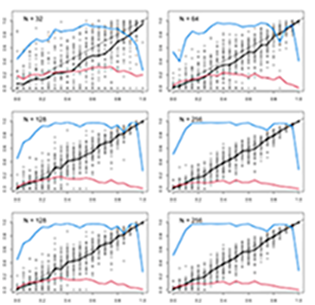
\includegraphics[width=0.95\linewidth]{new.fig.1.temp}

\singlespacing \textbf{Figure 1}. Temporary Fig. 1 showing lambda
patterns

\newpage

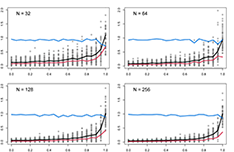
\includegraphics[width=0.95\linewidth]{new.fig.2.temp}

\singlespacing \textbf{Figure 2}. Temporary Fig. 2 showing kappa
patterns

\newpage

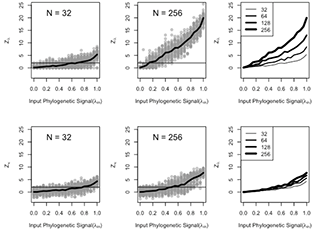
\includegraphics[width=0.95\linewidth]{new.fig.3.temp}

\singlespacing \textbf{Figure 3}. Temporary Fig. 3 showing z patterns

\newpage

\hypertarget{refs}{}
\leavevmode\hypertarget{ref-Felsenstein1985}{}%
1. J. Felsenstein, Phylogenies and the comparative method.
\emph{American Naturalist} \textbf{125}, 1--15 (1985).

\leavevmode\hypertarget{ref-HarveyPagel1991}{}%
2. P. H. Harvey, M. D. Pagel, \emph{The comparative method in
evolutionary biology} (Oxford University Press, 1991).

\leavevmode\hypertarget{ref-Grafen1989}{}%
3. A. Grafen, The phylogenetic regression. \emph{Philosophical
Transactions of the Royal Society of London B, Biological Sciences}
\textbf{326}, 119--157 (1989).

\leavevmode\hypertarget{ref-GarlandIves2000}{}%
4. T. J. Garland, A. R. Ives, Using the past to predict the present:
Confidence intervals for regression equations in phylogenetic
comparative methods. \emph{American Naturalist} \textbf{155}, 346--364
(2000).

\leavevmode\hypertarget{ref-Rohlf2001}{}%
5. F. J. Rohlf, Comparative methods for the analysis of continuous
variables: Geometric interpretations. \emph{Evolution} \textbf{55},
2143--2160 (2001).

\leavevmode\hypertarget{ref-ButlerKing2004}{}%
6. M. A. Butler, A. A. King, Phylogenetic comparative analysis: A
modeling approach for adaptive evolution. \emph{American Naturalist}
\textbf{164}, 683--695 (2004).

\leavevmode\hypertarget{ref-MartinsHansen1997}{}%
7. E. P. Martins, T. F. Hansen, Phylogenies and the comparative method:
A general approach to incorporating phylogenetic information into the
analysis of interspecific data. \emph{American Naturalist} \textbf{149},
646--667 (1997).

\leavevmode\hypertarget{ref-OMeara_et_al2006}{}%
8. B. C. O'Meara, C. Ane, M. J. Sanderson, P. C. Wainwright, Testing for
different rates of continuous trait evolution using likelihood.
\emph{Evolution} \textbf{60}, 922--933 (2006).

\leavevmode\hypertarget{ref-RevellHarmon2008}{}%
9. L. J. Revell, L. J. Harmon, Testing quantitative genetic hypotheses
about the evolutionary rate matrix for continuous characters.
\emph{Evolutionary Ecology Research} \textbf{10}, 311--331 (2008).

\leavevmode\hypertarget{ref-Beaulieu_et_al2012}{}%
10. J. M. Beaulieu, D. C. Jhwueng, C. Boettiger, B. C. O'Meara, Modeling
stabilizing selection: Expanding the ornstein-uhlenbeck model of
adaptive evolution. \emph{Evolution} \textbf{66}, 2369--2383 (2012).

\leavevmode\hypertarget{ref-Adams2014b}{}%
11. D. C. Adams, A method for assessing phylogenetic least squares
models for shape and other high-dimensional multivariate data.
\emph{Evolution} \textbf{68}, 2675--2688 (2014).

\leavevmode\hypertarget{ref-Adams2014a}{}%
12. D. C. Adams, A generalized Kappa statistic for estimating
phylogenetic signal from shape and other high-dimensional dultivariate
data. \emph{Systematic Biology} \textbf{63}, 685--697 (2014).

\leavevmode\hypertarget{ref-AdamsCollyer2018b}{}%
13. D. C. Adams, M. L. Collyer, Phylogenetic anova: Group-clade
aggregation, biological challenges, and a refined permutation procedure.
\emph{Evolution} \textbf{72}, 1204--1215 (2018).

\leavevmode\hypertarget{ref-Pagel1999}{}%
14. M. D. Pagel, Inferring the historical patterns of biological
evolution. \emph{Nature} \textbf{401}, 877--884 (1999).

\leavevmode\hypertarget{ref-Blomberg_et_al2003}{}%
15. S. P. Blomberg, T. Garland, A. R. Ives, Testing for phylogenetic
signal in comparative data: Behavioral traits are more labile.
\emph{Evolution} \textbf{57}, 717--745 (2003).

\leavevmode\hypertarget{ref-Revell_et_al2008}{}%
16. L. J. Revell, L. J. Harmon, D. C. Collar, Phylogenetic signal,
evolutionary process, and rate. \emph{Systematic Biology} \textbf{57},
591--601 (2008).

\leavevmode\hypertarget{ref-Abouheif1999}{}%
17. E. Abouheif, A method for testing the assumption of phylogenetic
independence in comparative data. \emph{Evolutionary Ecology Research}
\textbf{1}, 895--909 (1999).

\leavevmode\hypertarget{ref-Gittleman1990}{}%
18. J. L. Gittleman, M. Kot, Adaptation: Statistics and a null model for
estimating phylogenetic effects. \emph{Systematic Zoology} \textbf{39},
227--241 (1990).

\leavevmode\hypertarget{ref-Klingenberg2010}{}%
19. C. P. Klingenberg, N. A. Gidaszewski, Testing and quantifying
phylogenetic signals and homoplasy in morphometric data.
\emph{Systematic biology} \textbf{59}, 245--261 (2010).

\leavevmode\hypertarget{ref-Munkemuller_et_al2012}{}%
20. T. Münkemüller\emph{et al.}, How to measure and test phylogenetic
signal. \emph{Methods in Ecology and Evolution} \textbf{3}, 743--756
(2012).

\leavevmode\hypertarget{ref-Pavoine2012}{}%
21. S. Pavoine, C. Ricotta, Testing for phylogenetic signal in
biological traits: The ubiquity of cross-product statistics.
\emph{Evolution: International Journal of Organic Evolution}
\textbf{67}, 828--840 (2012).

\leavevmode\hypertarget{ref-DinizFilho2012}{}%
22. J. A. F. Diniz-Filho, T. Santos, T. F. Rangel, L. M. Bini, A
comparison of metrics for estimating phylogenetic signal under
alternative evolutionary models. \emph{Genetics and Molecular Biology}
\textbf{35}, 673--679 (2012).

\leavevmode\hypertarget{ref-MolinaVenegas2017}{}%
23. R. Molina-Venegas, M. A. Rodríguez, Revisiting phylogenetic signal;
strong or negligible impacts of polytomies and branch length
information? \emph{BMC evolutionary biology} \textbf{17}, 53 (2017).

\leavevmode\hypertarget{ref-Revell2010}{}%
24. L. J. Revell, Phylogenetic signal and linear regression on species
data. \emph{Methods in Ecology and Evolution} \textbf{1}, 319--329
(2010).

\leavevmode\hypertarget{ref-Freckleton_et_al2002}{}%
25. R. P. Freckleton, P. H. Harvey, M. Pagel, Phylogenetic analysis and
comparative data: A test and review of evidence. \emph{American
Naturalist} \textbf{160}, 712--726 (2002).

\leavevmode\hypertarget{ref-Cooper2010}{}%
26. N. Cooper, W. Jetz, R. P. Freckleton, Phylogenetic comparative
approaches for studying niche conservatism. \emph{Journal of
Evolutionary Biology} \textbf{23}, 2529--2539 (2010).

\leavevmode\hypertarget{ref-Bose2019}{}%
27. R. Bose, B. R. Ramesh, R. Pélissier, F. Munoz, Phylogenetic
diversity in the western ghats biodiversity hotspot reflects
environmental filtering and past niche diversification of trees.
\emph{Journal of Biogeography} \textbf{46}, 145--157 (2019).

\leavevmode\hypertarget{ref-Vandelook2019}{}%
28. F. Vandelook\emph{et al.}, Nectar traits differ between pollination
syndromes in balsaminaceae. \emph{Annals of Botany} \textbf{124},
269--279 (2019).

\leavevmode\hypertarget{ref-DeMeester2019}{}%
29. G. De Meester, K. Huyghe, R. Van Damme, Brain size, ecology and
sociality: A reptilian perspective. \emph{Biological Journal of the
Linnean Society} \textbf{126}, 381--391 (2019).

\leavevmode\hypertarget{ref-Pintanel2019}{}%
30. P. Pintanel, M. Tejedo, S. R. Ron, G. A. Llorente, A. Merino-Viteri,
Elevational and microclimatic drivers of thermal tolerance in andean
pristimantis frogs. \emph{Journal of Biogeography} \textbf{46},
1664--1675 (2019).

\leavevmode\hypertarget{ref-Su2019}{}%
31. G. Su, S. Villéger, S. Brosse, Morphological diversity of freshwater
fishes differs between realms, but morphologically extreme species are
widespread. \emph{Global ecology and biogeography} \textbf{28}, 211--221
(2019).

\end{document}
